\documentclass{article}\usepackage[]{graphicx}\usepackage[]{color}
%% maxwidth is the original width if it is less than linewidth
%% otherwise use linewidth (to make sure the graphics do not exceed the margin)
\makeatletter
\def\maxwidth{ %
  \ifdim\Gin@nat@width>\linewidth
    \linewidth
  \else
    \Gin@nat@width
  \fi
}
\makeatother

\definecolor{fgcolor}{rgb}{0.345, 0.345, 0.345}
\newcommand{\hlnum}[1]{\textcolor[rgb]{0.686,0.059,0.569}{#1}}%
\newcommand{\hlstr}[1]{\textcolor[rgb]{0.192,0.494,0.8}{#1}}%
\newcommand{\hlcom}[1]{\textcolor[rgb]{0.678,0.584,0.686}{\textit{#1}}}%
\newcommand{\hlopt}[1]{\textcolor[rgb]{0,0,0}{#1}}%
\newcommand{\hlstd}[1]{\textcolor[rgb]{0.345,0.345,0.345}{#1}}%
\newcommand{\hlkwa}[1]{\textcolor[rgb]{0.161,0.373,0.58}{\textbf{#1}}}%
\newcommand{\hlkwb}[1]{\textcolor[rgb]{0.69,0.353,0.396}{#1}}%
\newcommand{\hlkwc}[1]{\textcolor[rgb]{0.333,0.667,0.333}{#1}}%
\newcommand{\hlkwd}[1]{\textcolor[rgb]{0.737,0.353,0.396}{\textbf{#1}}}%
\let\hlipl\hlkwb

\usepackage{framed}
\makeatletter
\newenvironment{kframe}{%
 \def\at@end@of@kframe{}%
 \ifinner\ifhmode%
  \def\at@end@of@kframe{\end{minipage}}%
  \begin{minipage}{\columnwidth}%
 \fi\fi%
 \def\FrameCommand##1{\hskip\@totalleftmargin \hskip-\fboxsep
 \colorbox{shadecolor}{##1}\hskip-\fboxsep
     % There is no \\@totalrightmargin, so:
     \hskip-\linewidth \hskip-\@totalleftmargin \hskip\columnwidth}%
 \MakeFramed {\advance\hsize-\width
   \@totalleftmargin\z@ \linewidth\hsize
   \@setminipage}}%
 {\par\unskip\endMakeFramed%
 \at@end@of@kframe}
\makeatother

\definecolor{shadecolor}{rgb}{.97, .97, .97}
\definecolor{messagecolor}{rgb}{0, 0, 0}
\definecolor{warningcolor}{rgb}{1, 0, 1}
\definecolor{errorcolor}{rgb}{1, 0, 0}
\newenvironment{knitrout}{}{} % an empty environment to be redefined in TeX

\usepackage{alltt}
\usepackage{Sweave}
\usepackage{float}
\usepackage{graphicx}
\usepackage{tabularx}
\usepackage{siunitx}
\usepackage{mdframed}
\usepackage{natbib}
\bibliographystyle{..//refs/styles/besjournals.bst}
\usepackage[small]{caption}
\setkeys{Gin}{width=0.8\textwidth}
\setlength{\captionmargin}{30pt}
\setlength{\abovecaptionskip}{0pt}
\setlength{\belowcaptionskip}{10pt}
\topmargin -1.5cm        
\oddsidemargin -0.04cm   
\evensidemargin -0.04cm
\textwidth 16.59cm
\textheight 21.94cm 
&\pagestyle{empty} %comment if want page numbers
\parskip 0pt
\renewcommand{\baselinestretch}{1.5}
\parindent 10pt

\newmdenv[
  topline=true,
  bottomline=true,
  skipabove=\topsep,
  skipbelow=\topsep
]{siderules}
\usepackage{lineno}
\linenumbers
\IfFileExists{upquote.sty}{\usepackage{upquote}}{}
\begin{document}
\title{Hysteranthy Outline}

\section{Abstract}
\section{Introduction}
\begin{framed}
\textit{
"But green's the color of Spring\\
And green can be cool and friendly-like\\
And green can be big like an ocean, or important\\
Like a mountain, or tall like a tree"\\
It's Not Easy Being Green, Kermit the Frog}
\end{framed}
\par
Green is the color of spring, but a keen observer walking the Eastern deciduous forests early in the season would readily notice that it is often the subtle reds and yellows of emerging tree flowers that are the first harbingers of the season. Why does spring flowering proceeds leaf development in some woody species, while in others, it is leaf expansion that occurs first? Flowering before leafout, a trait refered to as hysteranthy \citep{}, protanthy \citep{} or precocious flowering \citep{} has been a feature of temperate decidious forest recognized and explained by botanists and ecologists for over a century \citep{}. Formulated generally, hysteranthy is classically explained to be an adaptation associated with wind pollinated tree species allowing for increase pollination effciency\citep{}, as the leafless state minimized physical barriers to pollen transfer \citep{} and increases wind speeds through the canopy, expanding pollen dispersal ranges\citep{}. This hypothesis has been carried in the ecological literature several lines of compelling indirect evidence. (Find Whitehead papers on pollen flow: Tauber 1965). Milleron and colleagues \citeyear{} demonstrated the prevelance of pollen interception by non-reproductive structes and the decrease in pollen dispersal distances after the return of and understory to a beech-oak forest following grazing exclusion. (perhaps expand this)
\par
But hysteranthy increasing pollination effeciency should also be considered for entomophilous species as well. Janzen \citeyear{} argues that hysteranthous flowering would increase flower visability and reduce flight path impediments for insect pollinators. In fact, many of iconic flowering trees, such as the cherry blossoms and magnolias, are hysteranthous and insect pollinated. The studies that address wind speed through the canopy seem only to consider hysteranthy as adaptive for large canopy species, (but maybe there is a better source I think perhaps spurr and barnes??), but do we truly find this phenological trait more commonly in tall trees very understory shrubs. The hypothesizes also imply hysteranthy is common in temperate diciduous forests, but how common? Might there be other trait more clearly associated with hysteranthy?
\par
(Were to define phenology)(Work this out more) Another hypothsis that can be found in the literature is an extension of the the theory surround early flowering in general. Early season flowering will maximize the time for seed development or germination \citep{Bolmgren08} and adaquate dispersal \citep{} may allow for escape from seed preditors\citep{}, And trees, which store ccarbohydrate between the season, seem to escape the growth vs. reproduction tradeoff found in the flowering literature regarding annual plants \citep{}. (not sure if this is important or could phrase it better.) In general, spring phenological advances for both floral and foliate  are constrained by the risk of damage by late spring frosts. It has been suggested that this stabalizing selection in stronger on foliar phenology (Jess Savage) as the cost of damage to the photosynthesithic capacity is greater than damage to the a year of reproduction in long lived organism such as trees. If floral phenology is independant of foliar, it maybe the combination of this differential selective pressure and selection for early flowering that produces hysteranthous patterning, and hysteranthy does not neccisairly have an adaptive function in and of itself.
\par
We know of no systematic study that has evaluated the merrit of the proposed associations or the prevelance of hysterany in the Temperate North American Flora-- Despite long history and increased interest in the study of phenology, timing of annual life cycle eventy,  to our knowledge, there have been no empircal studies, largely because floral and foliate phenoloy have long been treated seperatedly.
\par
in this paper we will...

. We investigated the prevelance and trait associations of hysteranthous flowering.\\
Hypothesis: Associated with wind pollination, and height. Also will test other biological relevant traits and the null hypothesis.\\
Alternative:Hysteranthy is an adapation for early flowering so fruit can mature and disperse. Flowers are less constrained than leaves by frost.

\section{Methods}
\subsection{Data and data preparation}
We obtained Flora-foliate sequence descriptions and all other trait descriptions from Michigan Trees and Michigan Shrubs and Vines.  The data sources provided verbal descriptions of floral-foliate sequences, which we coded as a binary resposponse. Descritions describing "flowers before leaves" or "flowers before or with leaves" were coded as hysteranthous and "flowers with leaf", "flowers with or after leaves" and "flowers after leaves" were coded as non-hysteranthous. We then selected species traits that have been previously implicated in exisiting hysteranthy hypothesizes (pollination syndrome,heigh class, dispersal phenology) and added additional biologically relevant traits (shade tolerance, flower type). All other traits of interest were also coded into bianary predictors: For pollination syndrome, species were classifed as (animal/wind. Ambophilous species such as those of the genus \textit{Salix} were classified as animal pollinated. For height class, species were classified as tree/shrub, with species with maximum height below or equalk to 15 meters classified as a shrub and above 15 meters as a tree. Shade tolerance was extracted from verbal descriptions, where "very shade tolerant","shade tolerant", and "moderately shade tolerant" were classified as "tolerant" and descriptions "shade intolerant" and "very shade intolerant" were classified as "intolerant". Dispersal phenology was classified as either "early season" or "late season", with species whose average month of dispersal falling before or at the mean of the dataset (mid August) classified as"early" and those after this time as "late". Flowers were classfied as either "unisexual or bisexual. We obtain hysteranthy classifications for 138 species, but only complete trait data for the 126 species used in the analysis. 
\par
To control for phylogenetic structure in our response variable, we utalized a published, rooted, angosperm phylogeny \citep{Zanne et al} and pruned it to match out data. 22 species which were not contain in our data but not in the phylogeny were added back into the tree randomly at the genus level nodes. We estimated the node ages of the tree using the mean lengths method \citep{Britton2002}. (Shoudld we interate the random design to get a maximum likelihood tree as nacho suggested)

\subsection{statistical analysis}
Using the brms pack interface between R and STAN, we developed a bayesian nonlinear mixed model to predict the likelihood a species is hysteranthous based on our predictors with phylogeny as the random effect to control for phylogenetic structure in the data. \\
\begin{equation}
Y_h_y_s_t_(_0_,_1_)=bx_p_o_l+bx_h_e_i_g_h_t+bx_d_i_s_p+bx_t_o_l+bx_f_l_o_w+(1|phyo)\\
\end{equation}
\par The full model and posterior predictive distribution can be viewd in the suppliment?
\par Maybe we compared this model to a plgs model

\section{Results}
\subsection{prevelence of hysteranthy}
49/138 species we looked at were hysteranthous\\
103/138  species are hysteranthous or synanthous\\ (should I report these out of the 126 I had full data for?)

\subsection{Trait associations}
There was a weak phylogenetic structure to hysteranthy (find it in brms, but you can use it from plgs)
Wind pollination and early fruit dispersal significantly increased the likelihood that a species will be hysteranthous.\\
Height class had no effect and was not significant. Shade intolerance increased likelihood of hysteranthy, but was not statistically significant.\\
Unisexual flowers also increased the likelihood of hsyteranthy, but was not statistically significant
\subsection{Model Comparision}
If neccisary

\section{Discussion}
Hypothesis is supported (both).\\
Classification may vary based on personal interpretation (eg silvics) or vary annually, or over population\\
Dont know what structures these paterns (external, internal)
related through resources, genetic pathways? and perhaps function (hysteranthy)
What will happen when climate changes
Phenology researchers need to consider flower and leaves together.

\section{Figures}

\begin{table}[H]
\begin{tabular}{|c|c|c|c|c|}
\hline
 &Estimate&Error&Lower CI& Upper CI\\
 \hline
Intercept&1.36&1.73&-2.04&4.93\\
\hline
Pollination syndrome&5.47&2.24&1.63&10.33\\
\hline
Height class&-0.10&1.78&-3.67&3.59\\
\hline
Fruiting time&-8.59&2.71&-14.39&-3.83\\
\hline
Shade tolerance&-1.87&1.59&5.38&0.97\\
\hline
Flower type&-1.59&1.81&-5.32&1.98\\
\hline

\end{tabular}
\end{table}


\begin{figure}[H]
 \fbox{ 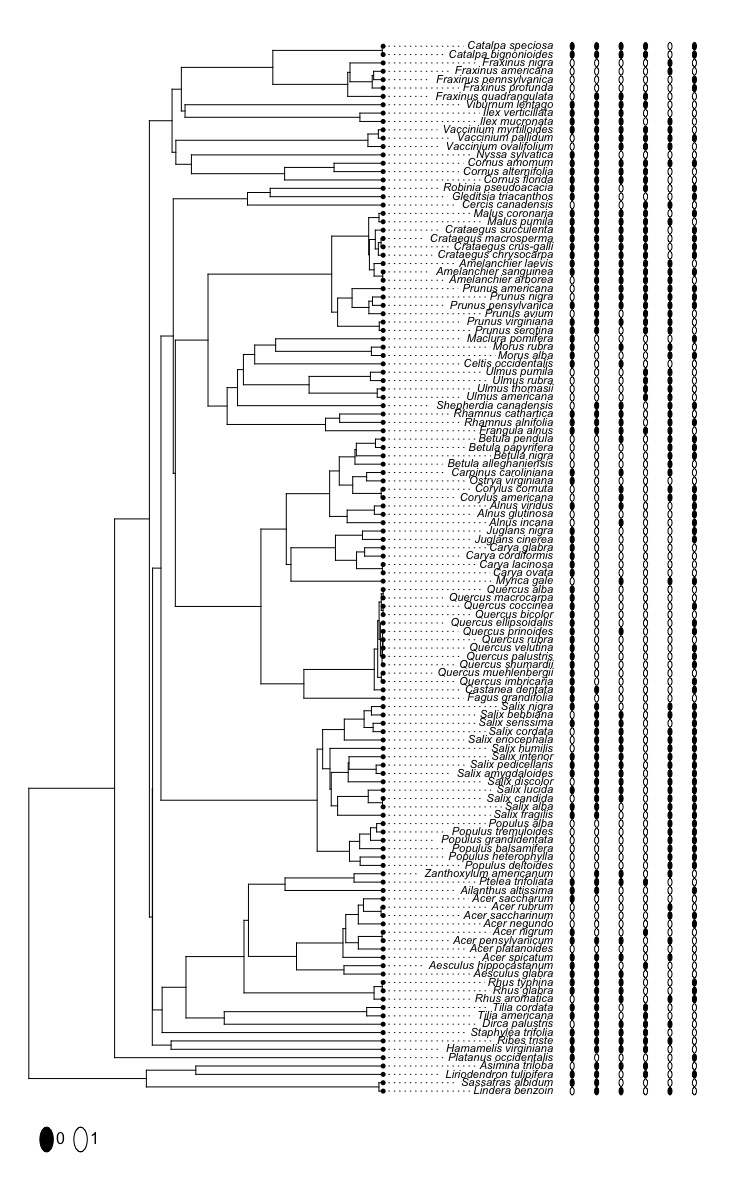
\includegraphics[width=12cm,height=12cm, keepaspectratio]{tree1.jpeg}} 
  \caption{This is my phylogeny, next to it all all the traits, I will have to explain these and label them}
  \label{Tree}
\end{figure}\\
\begin{figure}[H]
 \fbox{ 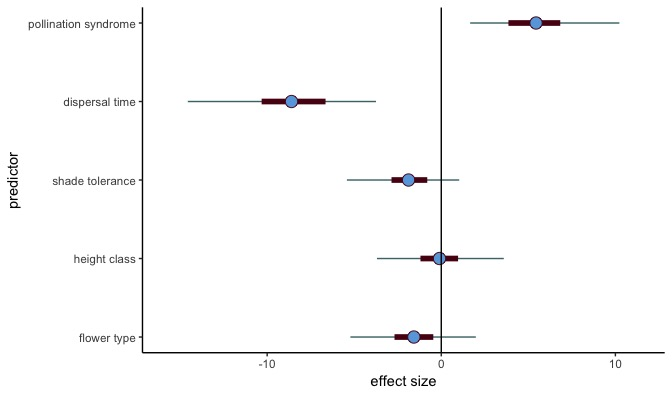
\includegraphics[width=\linewidth]{effect_plot2.jpeg}} 
  \caption{The effect size and significantce for each predictor, I'll explain this more too}
  \label{Effect sizes}
\end{figure}

\section{Suppliment}
full model with interactions
pp_checks?

\end{document}
